% \clearpage
\chapter{ТРАНСЛЯЦИЯ AST}

Трансляция AST осуществляется с помощью обхода дерева в глубину, что иллюстрирует следующее изображение[\ref{pass:compile-c:dfs-diag}]:

\begin{figure}[h!]
    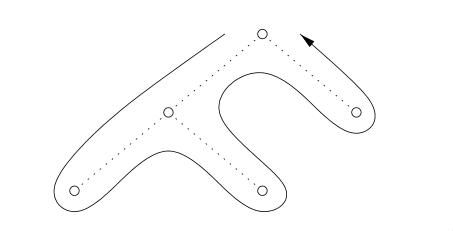
\includegraphics[width=0.6\linewidth]{tree-dfs.png}
    \centering
    \caption{Обход в глубину}
    \label{pass:compile-c:dfs-diag}
\end{figure}
\FloatBarrier

\section{Визуализация AST: Трансляция в dot}
\label{pass:compile-dot}

Можно визуализировать AST путем трансляции его к языку \textquote{dot} утилиты graphviz.
Трансляция выполнена в виде рекурсивного обхода AST аналогично трансляции в Си рассмотренной ранее[\ref{pass:compile-c}].
Примеры функции трансляции приведены [\ref{extras:compile-graphviz}].

Организуем код в виде функции единицы трансляции и тестируем:

\lstinputlisting[language={c},caption={Код теста визуализации}]{listings/translation/ast_vis/graphviz_test.c}

% \clearpage
Из входного файла \verb|ex_gv.c|:

\begin{lstlisting}[language=c, caption={ex\_gv.c}]
struct S {
    int x;
    Foo *foo;
};
\end{lstlisting}

Получаем файл \verb|ex_out.dot|:

\lstinputlisting[language={bash},caption={ex\_out.dot}]{listings/translation/ast_vis/ex_out.dot}
\clearpage
Применяем к нему движок dot фреймворка graphviz
\begin{lstlisting}[language=bash]
dot -Tpng sandbox/ex_out.dot -o build/ex_out.png
\end{lstlisting}

Получаем схему[\ref{graphviz:struct}]:

\begin{figure}[h!]
    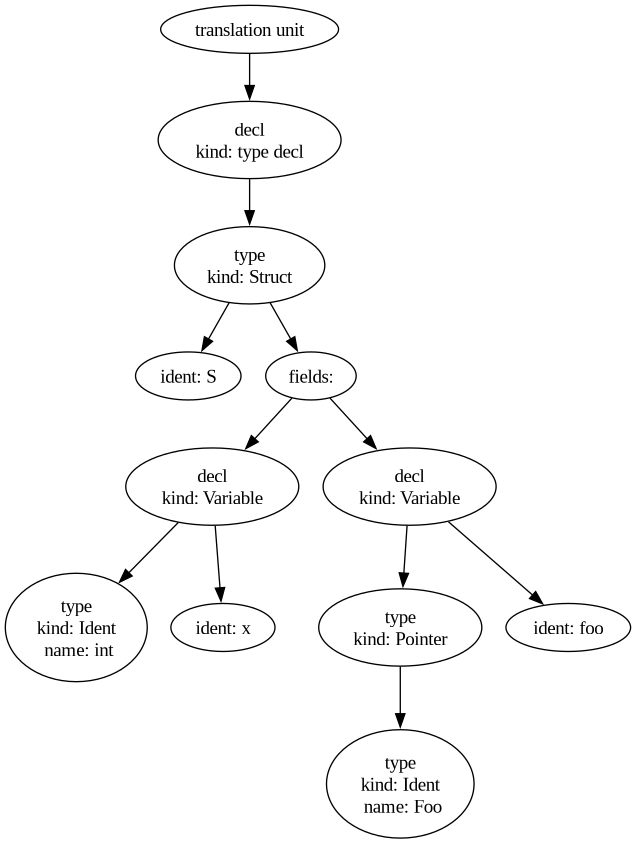
\includegraphics[width=\textwidth,height=0.7\textheight,keepaspectratio]{ex_out.png}
    \centering
    \caption{Синтаксическое дерево программы Си}
    \label{graphviz:struct}
\end{figure}

% \begin{figure}
%     \centering
%     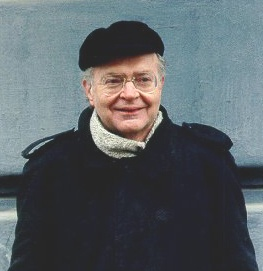
\includegraphics[width=0.6\linewidth]{images/knuth}
%     \caption{Knuth}
%     \label{fig:my_label4}
% \end{figure}

\clearpage
Теперь визуализируем следующее сложное определение переменных Си, где определения для трех переменных совмещены в одно.
\begin{lstlisting}[language=c]
int *(*x())[], y, *z;
\end{lstlisting}

После трансляции данного определения в язык dot с последующей компиляцией
получаем следующую схему AST выражения[\ref{graphviz:decl}]:

\begin{figure}[h!]
    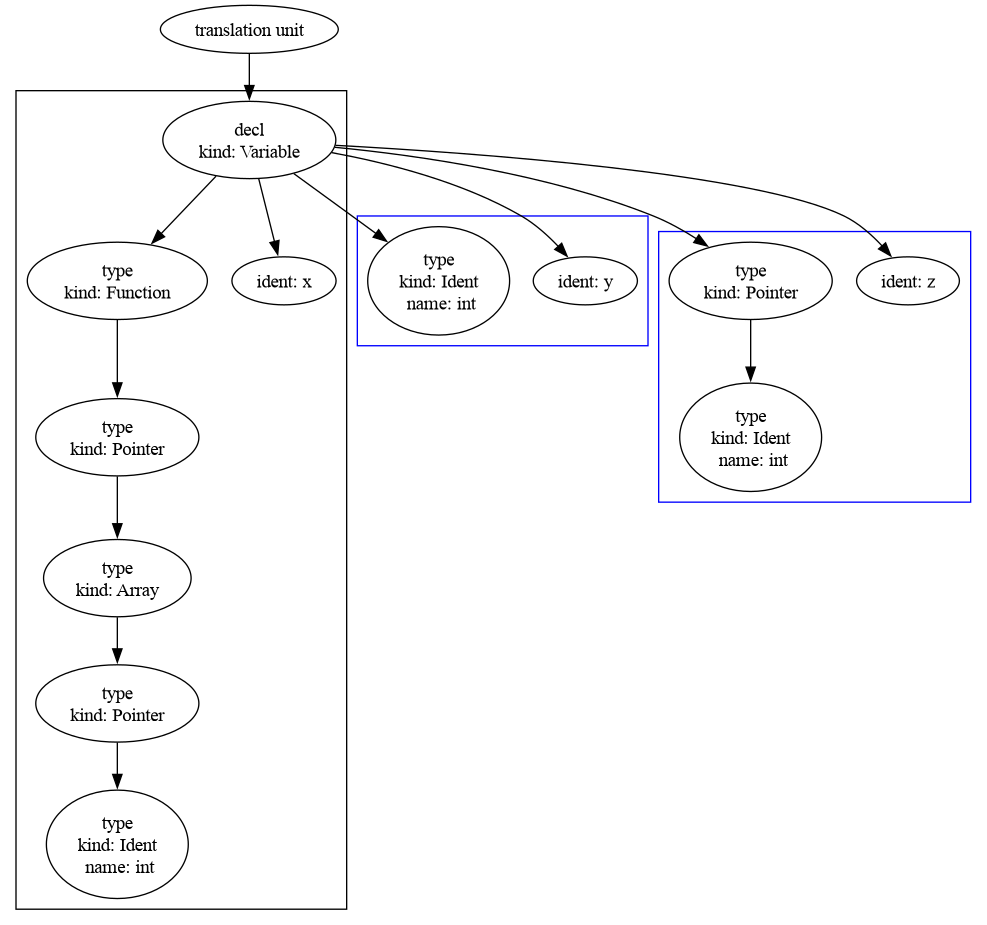
\includegraphics[width=\textwidth,height=\textheight,keepaspectratio]{ty_out.png}
    \centering
    \caption{AST сложного определения переменных Си}
    \label{graphviz:decl}
\end{figure}

\clearpage
Аналогично визуализируем выражение.
\begin{lstlisting}[language=c]
x = (a = a1) && b == c || d
\end{lstlisting}

После трансляции данного определения в язык dot с последующей компиляцией
получаем следующую схему AST выражения[\ref{graphviz:expr}]:
\begin{figure}[h!]
    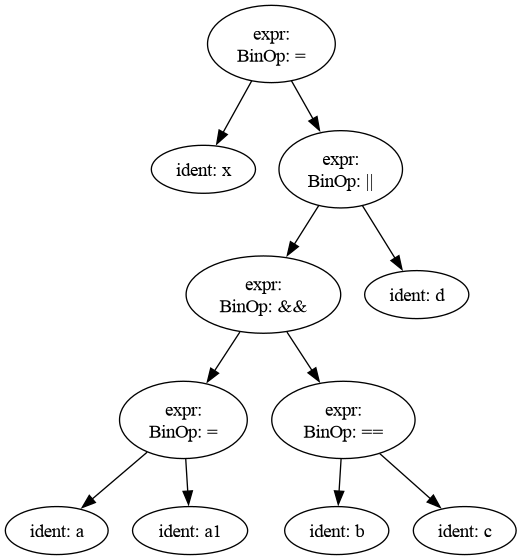
\includegraphics[width=0.8\textwidth]{expr_out.png}
    \centering
    \caption{AST выражения Си}
    \label{graphviz:expr}
\end{figure}

Таким образом данный функционал позволяет повысить наглядность структуры AST, что использовалось при отладке парсера, в частности парсера выражений, где можно ошибиться с порядком следования операторов.








\section{Трансляция AST в язык Си}
\label{pass:compile-c}


Рассмотрим как происходит процесс трансляции в язык Си. За это отвечает проход, выполненный в виде функции \hfill\break\verb|ec_translation_unit_ast_compile_c|.

\begin{lstlisting}[language=c, caption={Проход трансляции в язык Си}, label={pass:compile-c:compile-c-impl}]
void
ec_translation_unit_ast_compile_c(C_TranslationUnitData *self, StreamWriter *dst_sw) {
    auto fmt = string_formatter_default(dst_sw);
    ASSERT_OK(ec_ast_translation_unit_compile_c_fmt((EC_Ast_TranslationUnit *)self->tr_unit, &fmt, nullptr));
    ASSERT_OK(string_formatter_done(&fmt));
}
\end{lstlisting}

% Все, что данная функция делает это создает объект типа \verb|StringFormatter| с помощью выходного потока \verb|dst_sw| и передает его в основную функцию 
% трансляции \verb|ec_ast_translation_unit_compile_c_fmt|.

Данная функция является оберткой над основной функцией \newline \verb|ec_ast_translation_unit_compile_c_fmt|, применяющая интерфейс типа \verb|StringFormatter|.

Код основной функции привожу далее[\ref{pass:compile-c:compile-c-fmt-impl}]:

\begin{lstlisting}[language=c, caption={Функция трансляции типа Единицы Трансляции}, label={pass:compile-c:compile-c-fmt-impl}]
FmtError
ec_ast_translation_unit_compile_c_fmt(EC_Ast_TranslationUnit *tr_unit, StringFormatter *fmt, void *_) {
    auto items = tr_unit->items;
    for_in_range(i, 0, darr_len(items)) {
        auto item = *darr_get_T(EC_Ast_TrUnitItem *, items, i);
        if (item->kind == C_AST_NODE_KIND_DECL) {
            auto decl = (C_Ast_Decl *)item;
            if (decl->decl_kind == C_AST_DECL_KIND_EMPTY) {
                continue;
            }
            TRY(c_ast_decl_unparse_fmt(decl, fmt, nullptr));
            TRY(string_formatter_write(fmt, S("\n\n")));
        } else if (item->kind == C_AST_NODE_KIND_AT_DIRECTIVE) {
            auto dir = (EC_Ast_AtDirective *)item;
            TRY(ec_interpret_post_at_directive_fmt(dir, fmt, nullptr));
        } else {
            unreacheble();
        }
    }

    return FMT_ERROR(OK);
}
\end{lstlisting}


Данная функция в цикле проходится по всем корневым определениям и оставшимся директивам(в текущем прототипе только \verb|@post_include|),
печатая их с помощью типа \verb|StringFormatter| в выходной поток.

Трансляция определений производится обходом AST в глубину с помощью взаимно рекурсивных функций, заголовки которых приведены ниже[\ref{pass:compile-c:unparse-headers}]:

\begin{lstlisting}[language=c, caption={Заголовки функций трансляции AST в язык Си}, label={pass:compile-c:unparse-headers}]
FmtError
c_ast_ident_unparse_fmt(C_Ast_Ident *ident, StringFormatter *fmt, void *_);
FmtError
c_ast_expr_unparse_fmt(C_Ast_Expr *expr, StringFormatter *fmt, bool force_parens);
FmtError
c_ast_decl_unparse_fmt(C_Ast_Decl *decl, StringFormatter *fmt, void *_);
FmtError
c_ast_record_unparse_fmt(C_Ast_TypeRecord *record, StringFormatter *fmt, void *_);
FmtError
c_ast_struct_unparse_fmt(C_Ast_TypeStruct *_struct, StringFormatter *fmt, void *_);
FmtError
c_ast_union_unparse_fmt(C_Ast_TypeUnion *_union, StringFormatter *fmt, void *_);
FmtError
c_ast_type_unparse_fmt(C_Ast_Type *ty, StringFormatter *fmt, void *var_name, bool discard_leaf);
\end{lstlisting}

Реализация некоторых из них приведена в приложении[\ref{extras:unparse}].

Данные функции принимают элемент AST, объект типа \verb|StringFormatter| и дополнительные параметры.
Данный интерфейс позволяет производить трансляцию в любой абстрактный поток вывода, находящийся в форматоре \verb|fmt|.



\verb|@post_include| директивы интерпретируются следующей функцией[\ref{pass:compile-c:interpret-impl}]:

\begin{lstlisting}[language=c, caption={Функция трансляции директив}, label={pass:compile-c:interpret-impl}]
FmtError
ec_interpret_post_at_directive_fmt(EC_Ast_AtDirective *dir, StringFormatter *fmt, void *) {
    auto name = dir->name->name;
    if (str_eq(name, S("post_include"))) {
        ASSERT(dir->args && darr_len(dir->args) > 0);
        for_in_range(i, 0, darr_len(dir->args)) {
            auto arg = *darr_get_T(C_Ast_Literal *, dir->args, i);
            ASSERT(arg->lit_kind == C_AST_LITERAL_KIND_STRING);
            TRY(string_formatter_write_fmt(fmt, S("#include \"%s\"\n"), arg->l_str.t_str_lit->str));
        }
    } else {
        unreacheble();
    }

    return FMT_ERROR(OK);
}
\end{lstlisting}

Данная функций для каждого своего аргумента, который должен быть приведен в виде строкового литерала, печатает аналогичную \verb|#include| директиву препроцессора Си.

Таким образом производится трансляция AST в язык Си.

% Входной файл \verb|ex.c|
% \begin{code}
%   \inputminted[breaklines=true, xleftmargin=1em, linenos, frame=single,
%   framesep=10pt, fontsize=\footnotesize]
%   {c}{listings/translation/unparse/ex.c}
%   \label{ex.c}
% \end{code}

% Выходной файл \verb|ex\_out.c|
% \begin{code}
%   \inputminted[breaklines=true, xleftmargin=1em, linenos, frame=single,
%   framesep=10pt, fontsize=\footnotesize]
%   {c}{listings/translation/unparse/ex_out.c}
%   \label{ex_out.c}
% \end{code}

Итак на данном этапе был разобран функционал библиотеки позволяющий преобразовывать текст программы к синтаксическому дереву и обратно, 
т.е. выполнять сериализацию/десериализацию AST. Если сейчас последовательно применить лексический, грамматический разборы и затем транслировать дерево обратно в Си, то 
получатся практически идентичные файлы за исключением, может быть, кол-ва пробелов и переносов строк. 
Теперь вставленные между стадиями разбора и трансляции проходы будут отображены в выходном файле.
Данные этапы(проходы) модификации AST будут рассмотрены в следующей главе.